% begin module volumes-intro
\begin{frame}
\frametitle{Volumes}
\begin{center}
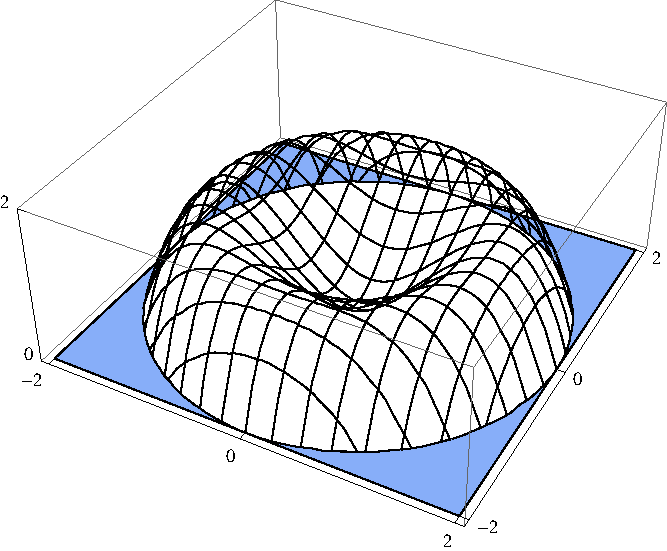
\includegraphics[height=6.5cm]{volumes/pictures/06-03-setup3d.pdf} %

We can use integration to find the volumes of certain solids.%
\end{center}
\end{frame}

\begin{frame}
\begin{columns}[c]
\column{.35\textwidth}
\only<handout:1| -1>{%
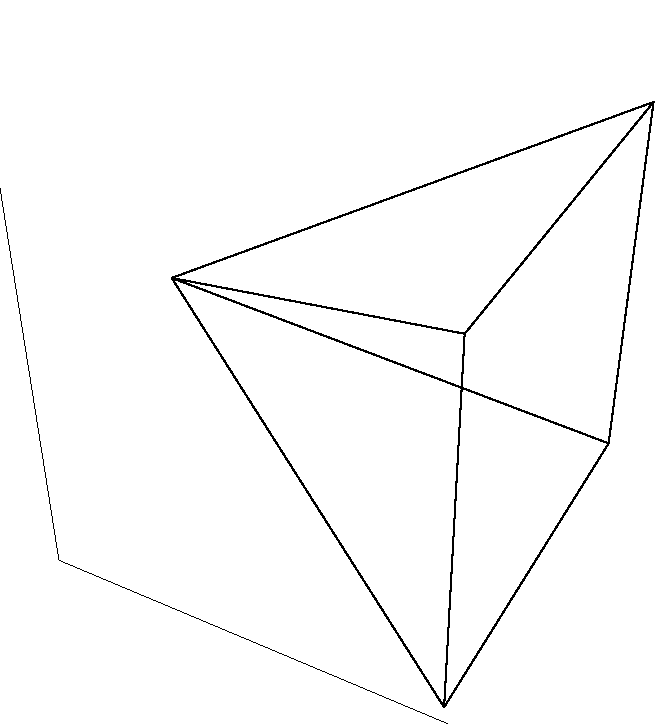
\includegraphics[height=4cm]{volumes/pictures/06-02-pyramida.pdf} %
}%
\only<handout:0| 2>{%
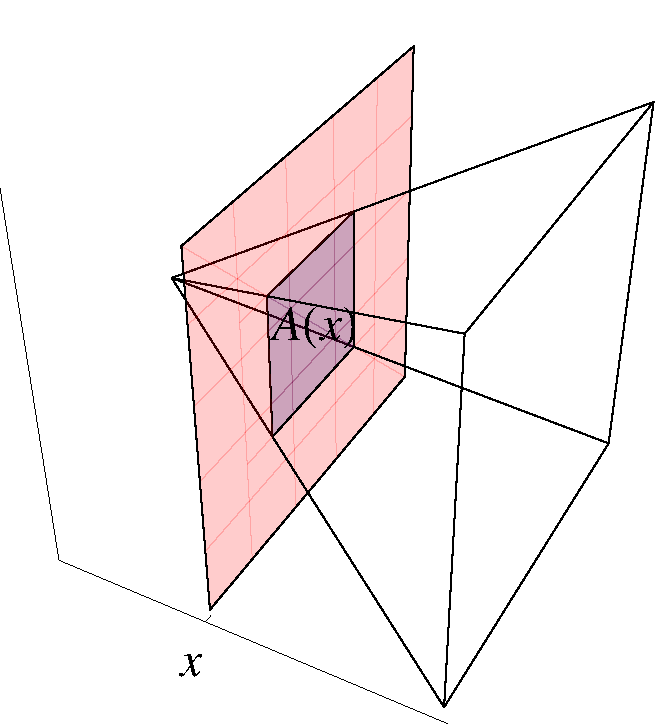
\includegraphics[height=4cm]{volumes/pictures/06-02-pyramidb.pdf}%
}%
\only<handout:0| 3>{%
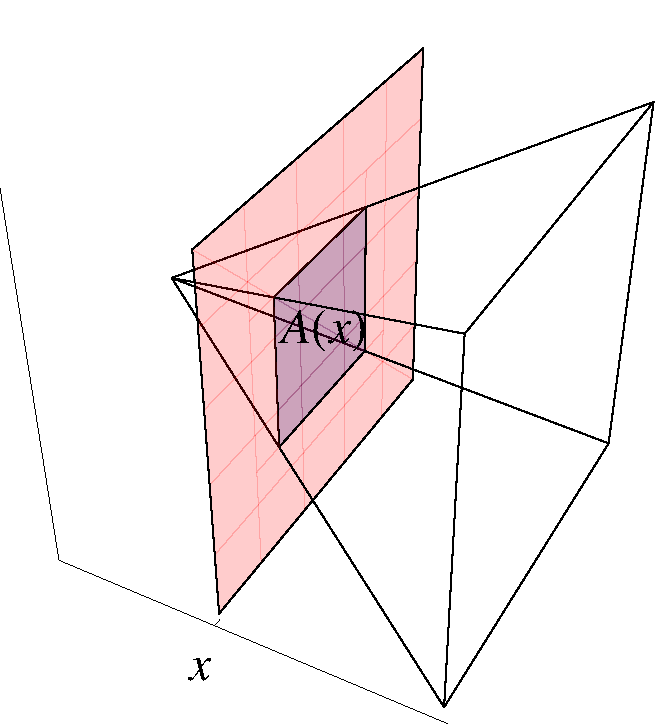
\includegraphics[height=4cm]{volumes/pictures/06-02-pyramidc.pdf}%
}%
\only<handout:0| 4>{%
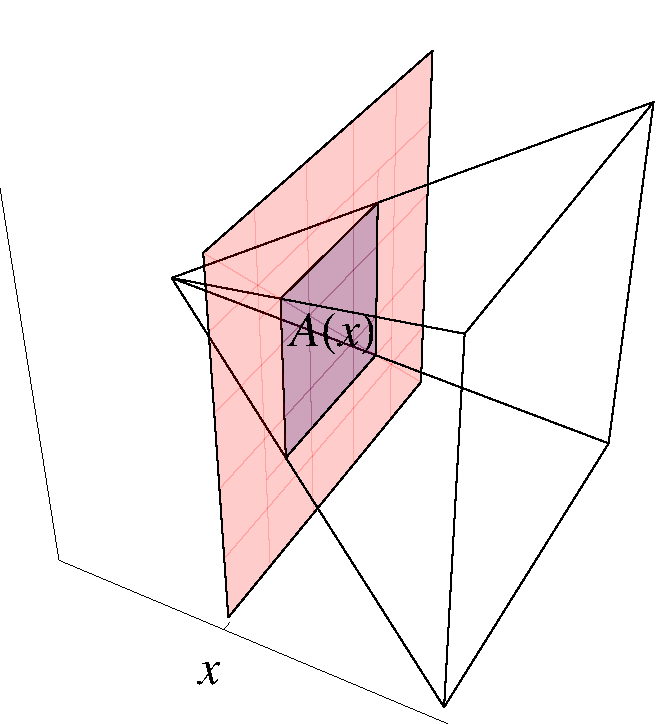
\includegraphics[height=4cm]{volumes/pictures/06-02-pyramidd.pdf}%
}%
\only<handout:2| 5>{%
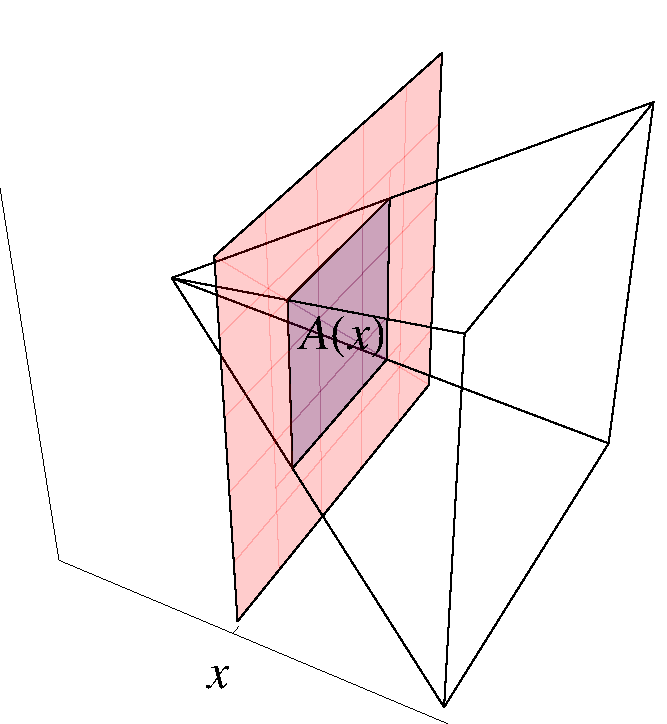
\includegraphics[height=4cm]{volumes/pictures/06-02-pyramide.pdf}%
}%
\only<handout:0| 6-7>{%
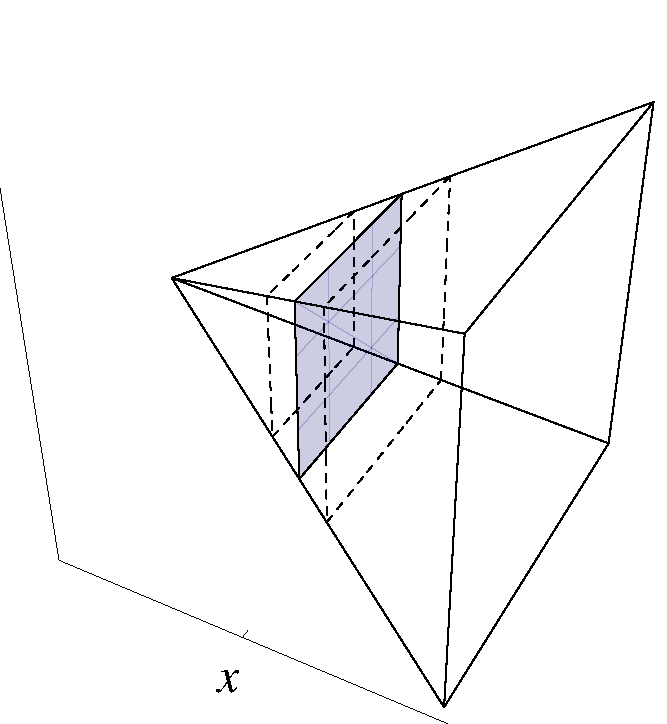
\includegraphics[height=4cm]{volumes/pictures/06-02-pyramidf.pdf}%
}%
\only<handout:3| 8->{%
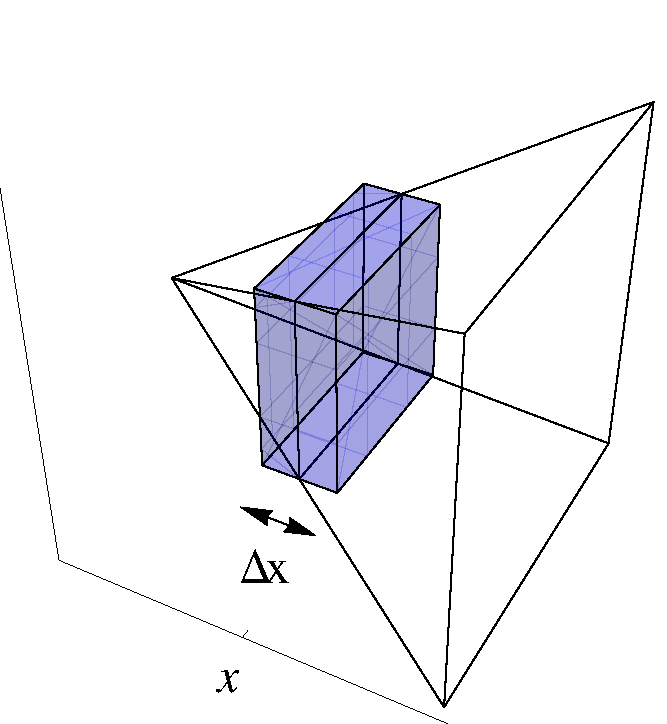
\includegraphics[height=4cm]{volumes/pictures/06-02-pyramidg.pdf}%
}%

\uncover<handout:3| 9->{Approx. volume of slab:}
\abovedisplayskip=1pt
\belowdisplayskip=1pt
\[
\uncover<handout:3| 9->{A(x^*)\Delta x}%
\]
\uncover<handout:3| 10->{Approx. volume of $S$:}
\abovedisplayskip=1pt
\belowdisplayskip=1pt
\[
\uncover<handout:3| 10->{V \approx \sum_{i=1}^n A(x_i^*)\Delta x}%
\]
\uncover<handout:3| 11->{Exact volume of $S$:}
\abovedisplayskip=1pt
\belowdisplayskip=1pt
\[
\uncover<handout:3| 11->{V = \lim_{n\to\infty}\sum_{i=1}^n A(x_i^*)\Delta x}%
\]
\column{.65\textwidth}
\begin{itemize}
\item  How do we find the volume of a solid $S$?
\item<handout:2-| 2->  Let $P_x$ be the plane perpendicular to the $x$-axis and passing through the point $x$.
\item<handout:2-| 2->  The intersection of $P_x$ with $S$ is called a cross-section.
\item<handout:2-| 2->  Let $A(x)$ be the area of this cross-section.
\item<handout:3| 6->  Consider the part of $S$ between two planes $P_{x_1}$ and $P_{x_2}$.
\item<handout:3| 7->  Approximate this part of $S$:
\item<handout:3| 7->  Pick a sample point $x^*$ between $x_1$ and $x_2$.  Use a solid that has the same constant cross-sectional area $A(x^*)$ between $x_1$ and $x_2$.
\item<handout:3| 8->  Let $\Delta x$ be the distance from $x_1$ to $x_2$.
\end{itemize}
\end{columns}
\end{frame}
% end module volumes-intro
